\documentclass[letter,11pt]{article}
\usepackage[margin=1.5cm]{geometry}
\usepackage{latexsym}
\usepackage{amsmath}
\usepackage{color}
\usepackage{graphicx}
\usepackage{amssymb}
\usepackage{alltt}
\usepackage{enumitem}
\usepackage{siunitx}
\usepackage{physics}
\usepackage{float}
\usepackage{bm}

\newenvironment{solution}{
    \vspace{0.16in} {\bf Solution:}
    
}{
	\vspace{0.16in}
}
\newcommand{\xx}{\bm{x}}
\newcommand{\vv}{\bm{v}}
\newcommand{\T}{T}
\newcommand{\RR}{\mathbb{R}}
\newcommand{\mub}{\bm{\mu}}
\newcommand{\thetab}{\bm{\theta}}
\newcommand{\Sigmab}{\bm{\Sigma}}
\newcommand{\m}[1]{\begin{bmatrix}#1\end{bmatrix}}
\newcommand{\N}{\mathcal{N}}
\newcommand{\PP}{\mathbb{P}}
\newcommand{\Dc}{\mathcal{D}}
\newcommand{\Nc}{\mathcal{N}}

%------------------------------------------------------

\begin{document}

\begin{center}
    {\bf \Large Math 189R problem set 5} \\
    \vspace{0.1in}
    Adam Guo \quad 2020-03-02
\end{center}

\begin{enumerate}
    \item \textbf{(Murphy 12.5 - Deriving the Residual Error for PCA)} It may be helpful to reference section 12.2.2 of Murphy.

    \begin{enumerate}
        \item Prove that \[\left\|\xx_i - \sum_{j=1}^k z_{ij}\vv_j\right\|^2 = \xx_i^\T\xx_i - \sum_{j=1}^k\vv_j^\T \xx_i\xx_i^\T \vv_j.\] Hint: first consider the case when $k=2$. Use the fact that $\vv_i^\T\vv_j$ is 1 if $i=j$ and 0 otherwise. Recall that $z_{ij} = \xx_i^\T\vv_j$.

        \begin{solution}
            \begin{align*}
                \left\| \xx_i - \sum_{j=1}^k z_{ij} \vv_j \right\|^2 &= (\xx_i - \sum_{j=1}^k z_{ij} \vv_j)^T (\xx_i - \sum_{j=1}^k z_{ij} \vv_j) \\
                &= \xx_i^T \xx_i - \xx_i \sum_{j=1}^k z_{ij} \vv_{j} - \left(\sum_{j=1}^k z_{ij} \vv_{j}^T\right) \xx_i + \sum_{j, l = 1}^k \vv_j^T z_{ij}^T z_{il} \vv_l \\
                &= \xx_i^T \xx_i - 2\sum_{j=1}^k z_{ij} \vv_j^T \xx_i + \sum_{j=1}^k \vv_j^T z_{ij}^T z_{ij} \vv_j \\
                &= \xx_i^T \xx_i - 2\sum_{j=1}^k \vv_j^T \xx_i \xx_i^T \vv_j + \sum_{j=1}^k \vv_j^T \xx_i \xx_i^T \vv_j \\
                &= \xx_i^T \xx_i - \sum_{j=1}^k \vv_j^T \xx_i \xx_i^T \vv_j
            \end{align*}
        \end{solution}

        \item Now show that \[J_k = \frac{1}{n}\sum_{i=1}^n \left(\xx_i^\T \xx_i - \sum_{j=1}^k\vv_j^\T \xx_i\xx_i^\T \vv_j\right) = \frac{1}{n}\sum_{i=1}^n \xx_i^\T\xx_i - \sum_{j=1}^k\lambda_j.\] Hint: recall that $\vv_j^\T \Sigmab \vv_j = \lambda_j\vv_j^\T\vv_j = \lambda_j$.

        \begin{solution}
            \begin{align*}
                J_k &= \frac1n \sum_{i=1}^n \left(\xx_i^T \xx_i - \sum_{j=1}^k \vv_j^T \xx_i \xx_i^T \vv_j\right) \\
                &= \frac1n \sum_{i=1}^n \xx_i^T \xx_i - \sum_{i=1}^k \vv_j^T \frac1n \sum_{j=1}^n \xx_i \xx_i^T \vv_j \\
                &= \frac1n \sum_{i=1}^n \xx_i^T \xx_i - \sum_{i=1}^n \vv_j^T \Sigmab \vv_j \\
                &= \frac1n \sum_{i=1}^n \xx_i^T \xx_i - \sum_{i=1}^k \lambda_j
            \end{align*}
        \end{solution}

        \item If $k=d$ there is no truncation, so $J_d=0$. Use this to show that the error from only using $k<d$ terms is given by \[J_k = \sum_{j=k+1}^d \lambda_j.\] Hint: partition the sum $\sum_{j=1}^d \lambda_j$ into $\sum_{j=1}^k \lambda_j$ and $\sum_{j=k+1}^d \lambda_j$.

        \begin{solution}
            \begin{align*}
                J_k &= \frac1n \sum_{i=1}^n \xx_i^T \xx_i - \sum_{j=1}^k \lambda_j \\
                &= \frac1n \sum_{i=1}^n \xx_i^T \xx_i - \sum_{j=1}^d \lambda_j + \sum_{j=k+1}^d \lambda_j
                \intertext{Since $J_d$ = 0,}
                0 &= \frac1n \sum_{i=1}^n \xx_i^T \xx_i - \sum_{i=1}^d \lambda_j
                \intertext{Thus,}
                J_k &= \sum_{j=k+1}^d \lambda_j
            \end{align*}
        \end{solution}
    \end{enumerate}

    \newpage

    % ----------------------------------

    \item \textbf{($\ell_1$-Regularization)} Consider the $\ell_1$ norm of a vector $\xx\in\RR^n$: \[\|\xx\|_1 = \sum_i |\xx_i|.\] Draw the norm-ball $B_k = \{\xx : \|\xx\|_1 \leq k\}$ for $k=1$. On the same graph, draw the Euclidean norm-ball $A_k = \{\xx : \|\xx\|_2 \leq k\}$ for $k=1$ behind the first plot. (Do not need to write any code, draw the graph by hand). Show that the optimization problem
    \begin{align*}
        \text{minimize: } & f(\xx)\\
        \text{subj. to: } & \|\xx\|_p \leq k
    \end{align*}
    is equivalent to
    \begin{align*}
        \text{minimize: } & f(\xx) + \lambda\|\xx\|_p
    \end{align*}
    (hint: create the Lagrangian). With this knowledge, and the plots given above, argue why using $\ell_1$ regularization (adding a $\lambda\|\xx\|_1$ term to the objective) will give sparser solutions than using $\ell_2$ regularization for suitably large $\lambda$.

    \begin{solution}
        \begin{figure}[H]
            \centering
            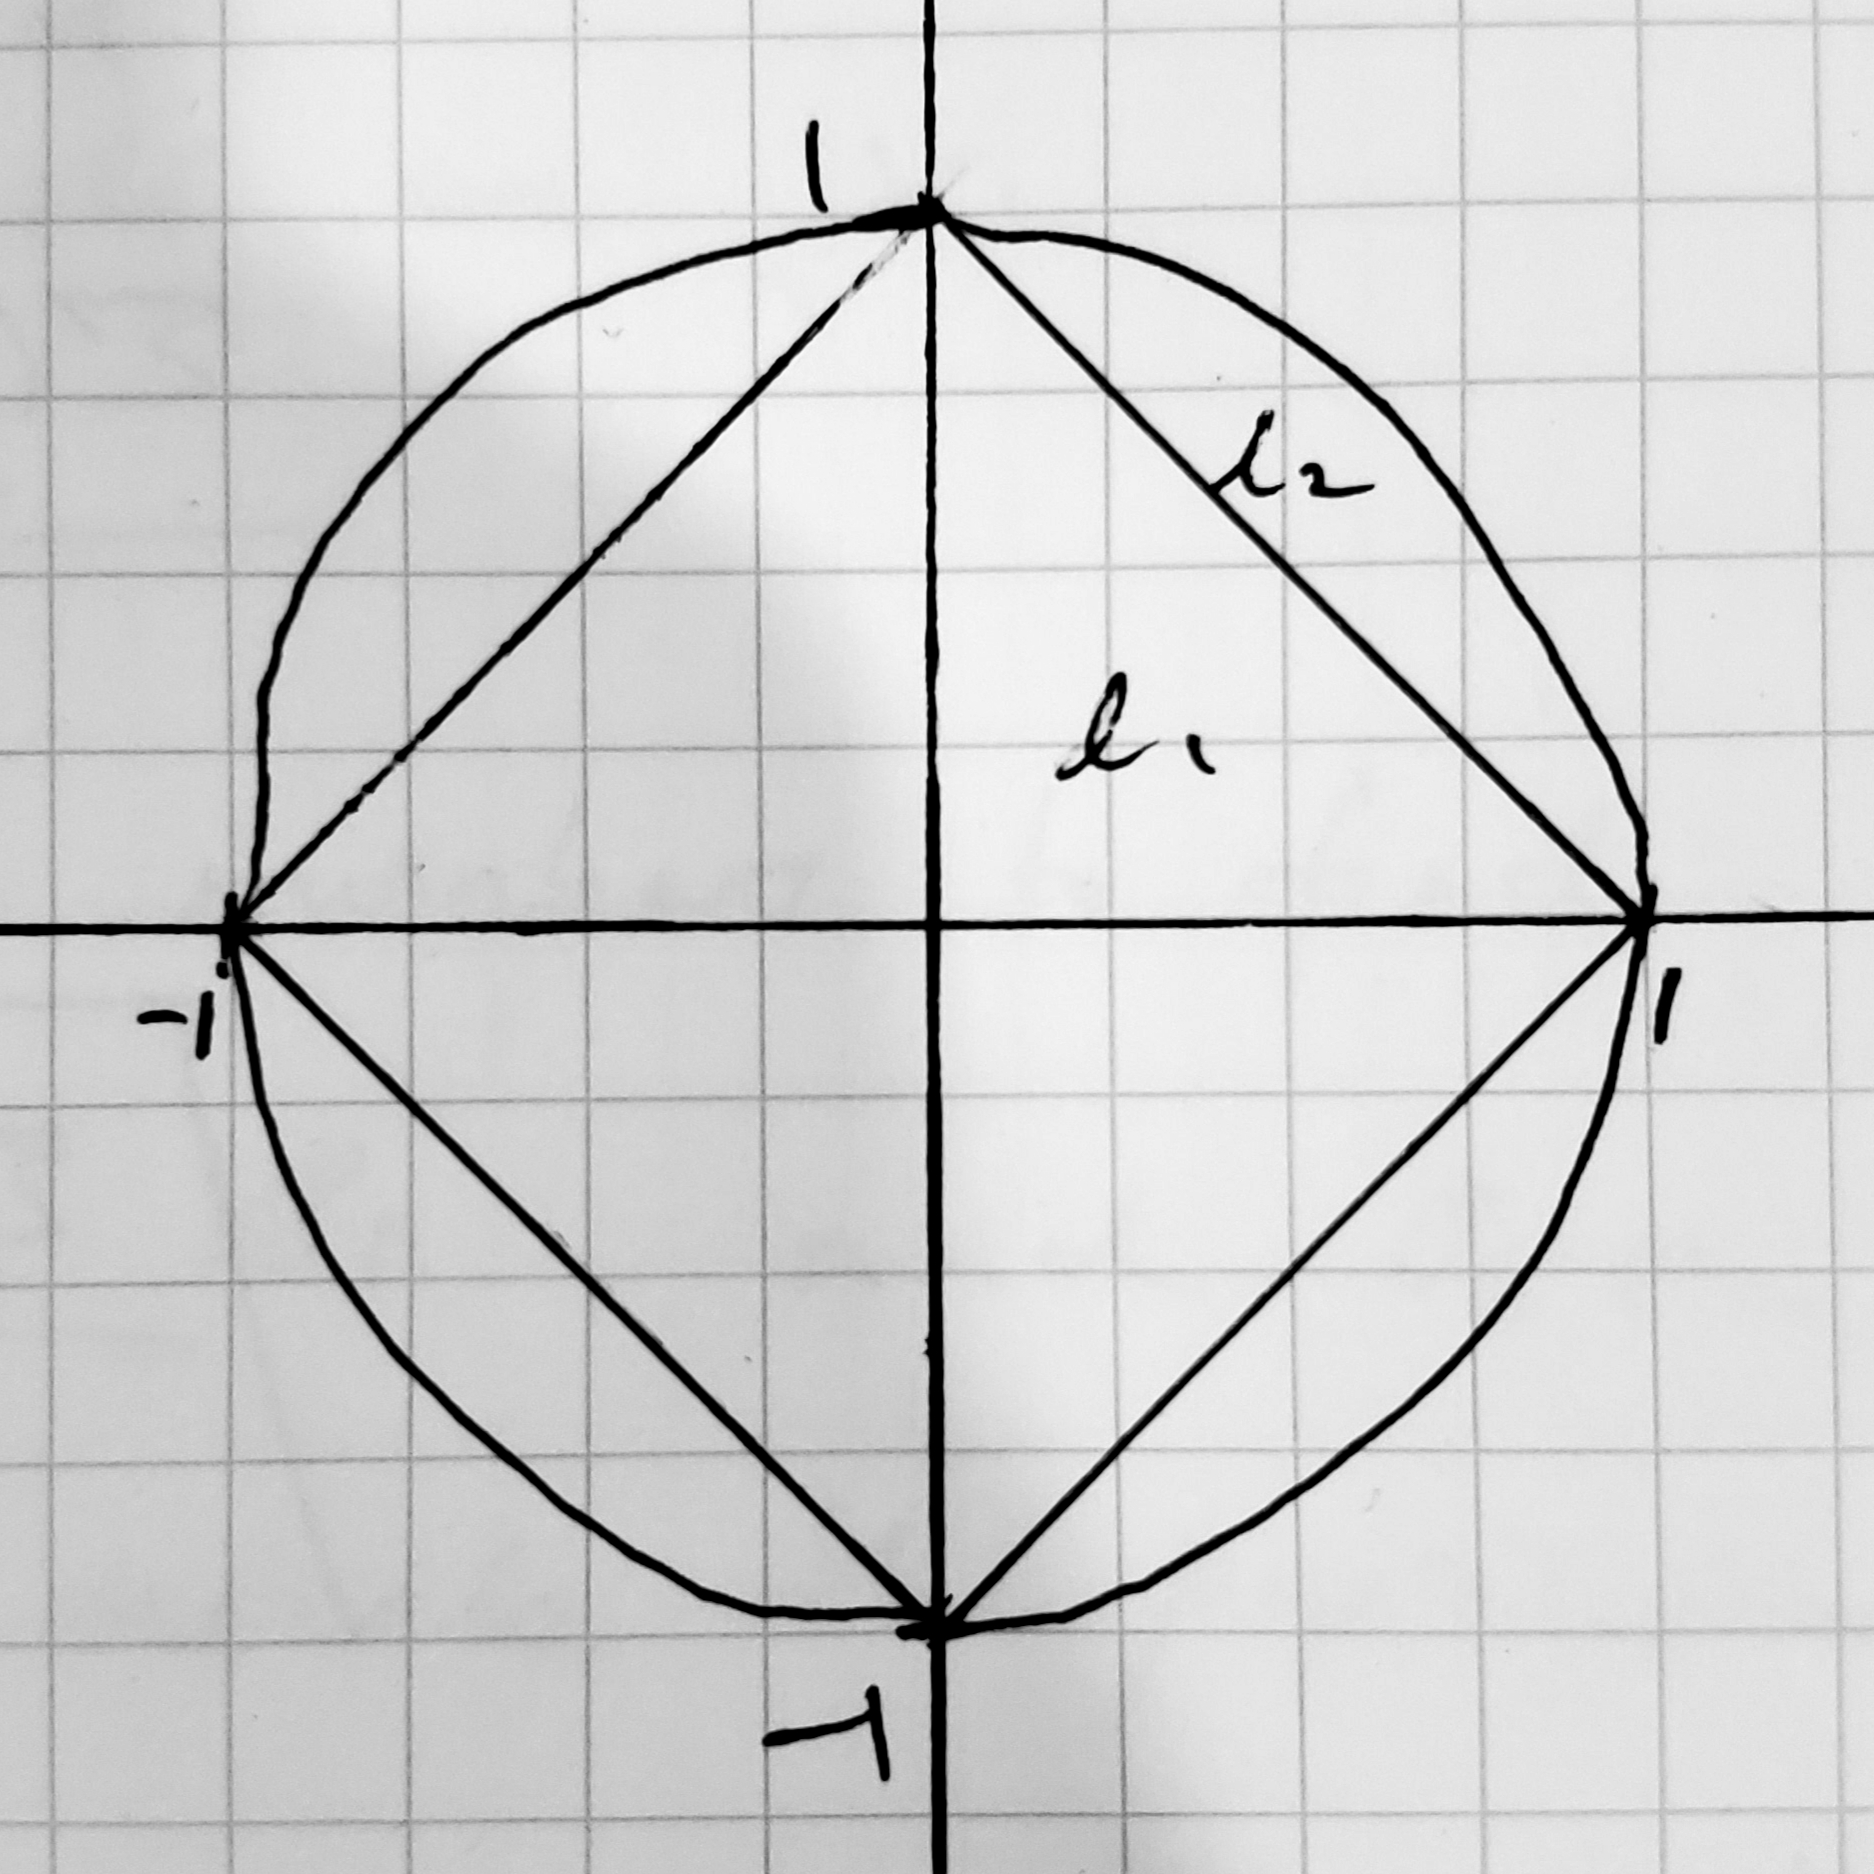
\includegraphics[width=6cm]{q2.jpg}
        \end{figure}

        The Lagrangian is given by \[\mathcal{L}(\xx, k) = f(x) + \lambda(\|\xx\|_p - k) = f(x) + \lambda \|\xx\|_p - \lambda k\] We want to minimise the Lagrangian to find the optimal solution for $\xx$. Since $\lambda k$ does not depend on $\xx$, this optimisation problem is equivalent to minimising $f(x) + \lambda\|\xx\|_p$. We see that the Euclidean distance from the origin to the ``corners'' of the $l_1$ ball than the distance to the edges. Hence, the optimal solution to the problem is more likely to first intersect with a corner of the $l_1$ ball than an edge. Compare this to the $l_2$ ball which is equidistant in Euclidean space to the origin, and therefore equally likely to first intersect the optimal solution at any point. Hence, using the $l_1$ ball is more likely to yield optimal solutions that lie on the $x$ or $y$ axes, and are therefore more sparse.
    \end{solution}

    \newpage

    % ----------------------------------

    \item \textbf{Extra credit (Lasso)} Show that placing an equal zero-mean Laplace prior on each element of the weights $\thetab$ of a model is equivalent to $\ell_1$ regularization in the Maximum-a-Posteriori estimate
    \begin{align*}
        \text{maximize: } & \PP(\thetab | \Dc) = \frac{\PP(\Dc | \thetab)\PP(\thetab)}{\PP(\Dc)}.
    \end{align*}
    Note the form of the Laplace distribution is \[\mathrm{Lap}(x|\mu,b) = \frac{1}{2b}\exp\left(-\frac{|x-\mu|}{b}\right)\] where $\mu$ is the location parameter and $b>0$ controls the variance. Draw (by hand) and compare the density $\mathrm{Lap}(x|0,1)$ and the standard normal $\Nc(x|0,1)$ and suggest why this would lead to sparser solutions than a Gaussian prior on each elements of the weights (which correspond to $\ell_2$ regularization).

    \begin{solution}
        Maximising $\PP(\thetab \mid \Dc)$ is equivalent to maximising the log likelihood, \[\ln \PP(\thetab \mid \Dc) = \ln \frac{\PP(\Dc \mid \thetab) \PP(\thetab)}{\PP(\Dc)} = \ln \PP(\Dc \mid \thetab) + \ln \PP(\thetab) - \PP(\Dc)\] Since $\PP(\Dc)$ does not depend on $\thetab$, this is equivalent to

        \begin{align*}
            \text{maximise:}& \quad\, \ln \PP(\Dc \mid \thetab) + \ln \PP(\thetab) \\
                &= \ln \PP(\Dc \mid \thetab) + \ln \left( \exp\left(-\frac{|\thetab_i|}{b}\right) \right) \\
                &= \ln \PP(\Dc \mid \thetab) + \ln \left(\prod_i \exp\left(-\frac{|\thetab_i|}{b}\right) \right) \\
                &= \ln \PP(\Dc \mid \thetab) + \sum_i \left(-\frac{|\thetab_i|}{b}\right) \\
                &= \ln \PP(\Dc \mid \thetab) - \frac{1}{b} \sum_i |\thetab_i| \\
                &= \ln \PP(\Dc \mid \thetab) - \lambda \|\thetab\|_1, \quad \lambda = \frac{1}{b}
        \end{align*}

        This is subsequently equivalent to \[\text{minimise: } -\ln \PP(\Dc \mid \thetab) + \lambda \|\thetab\|_1\] which is of the same form as $l_1$ regularisation.

        \begin{figure}[H]
            \centering
            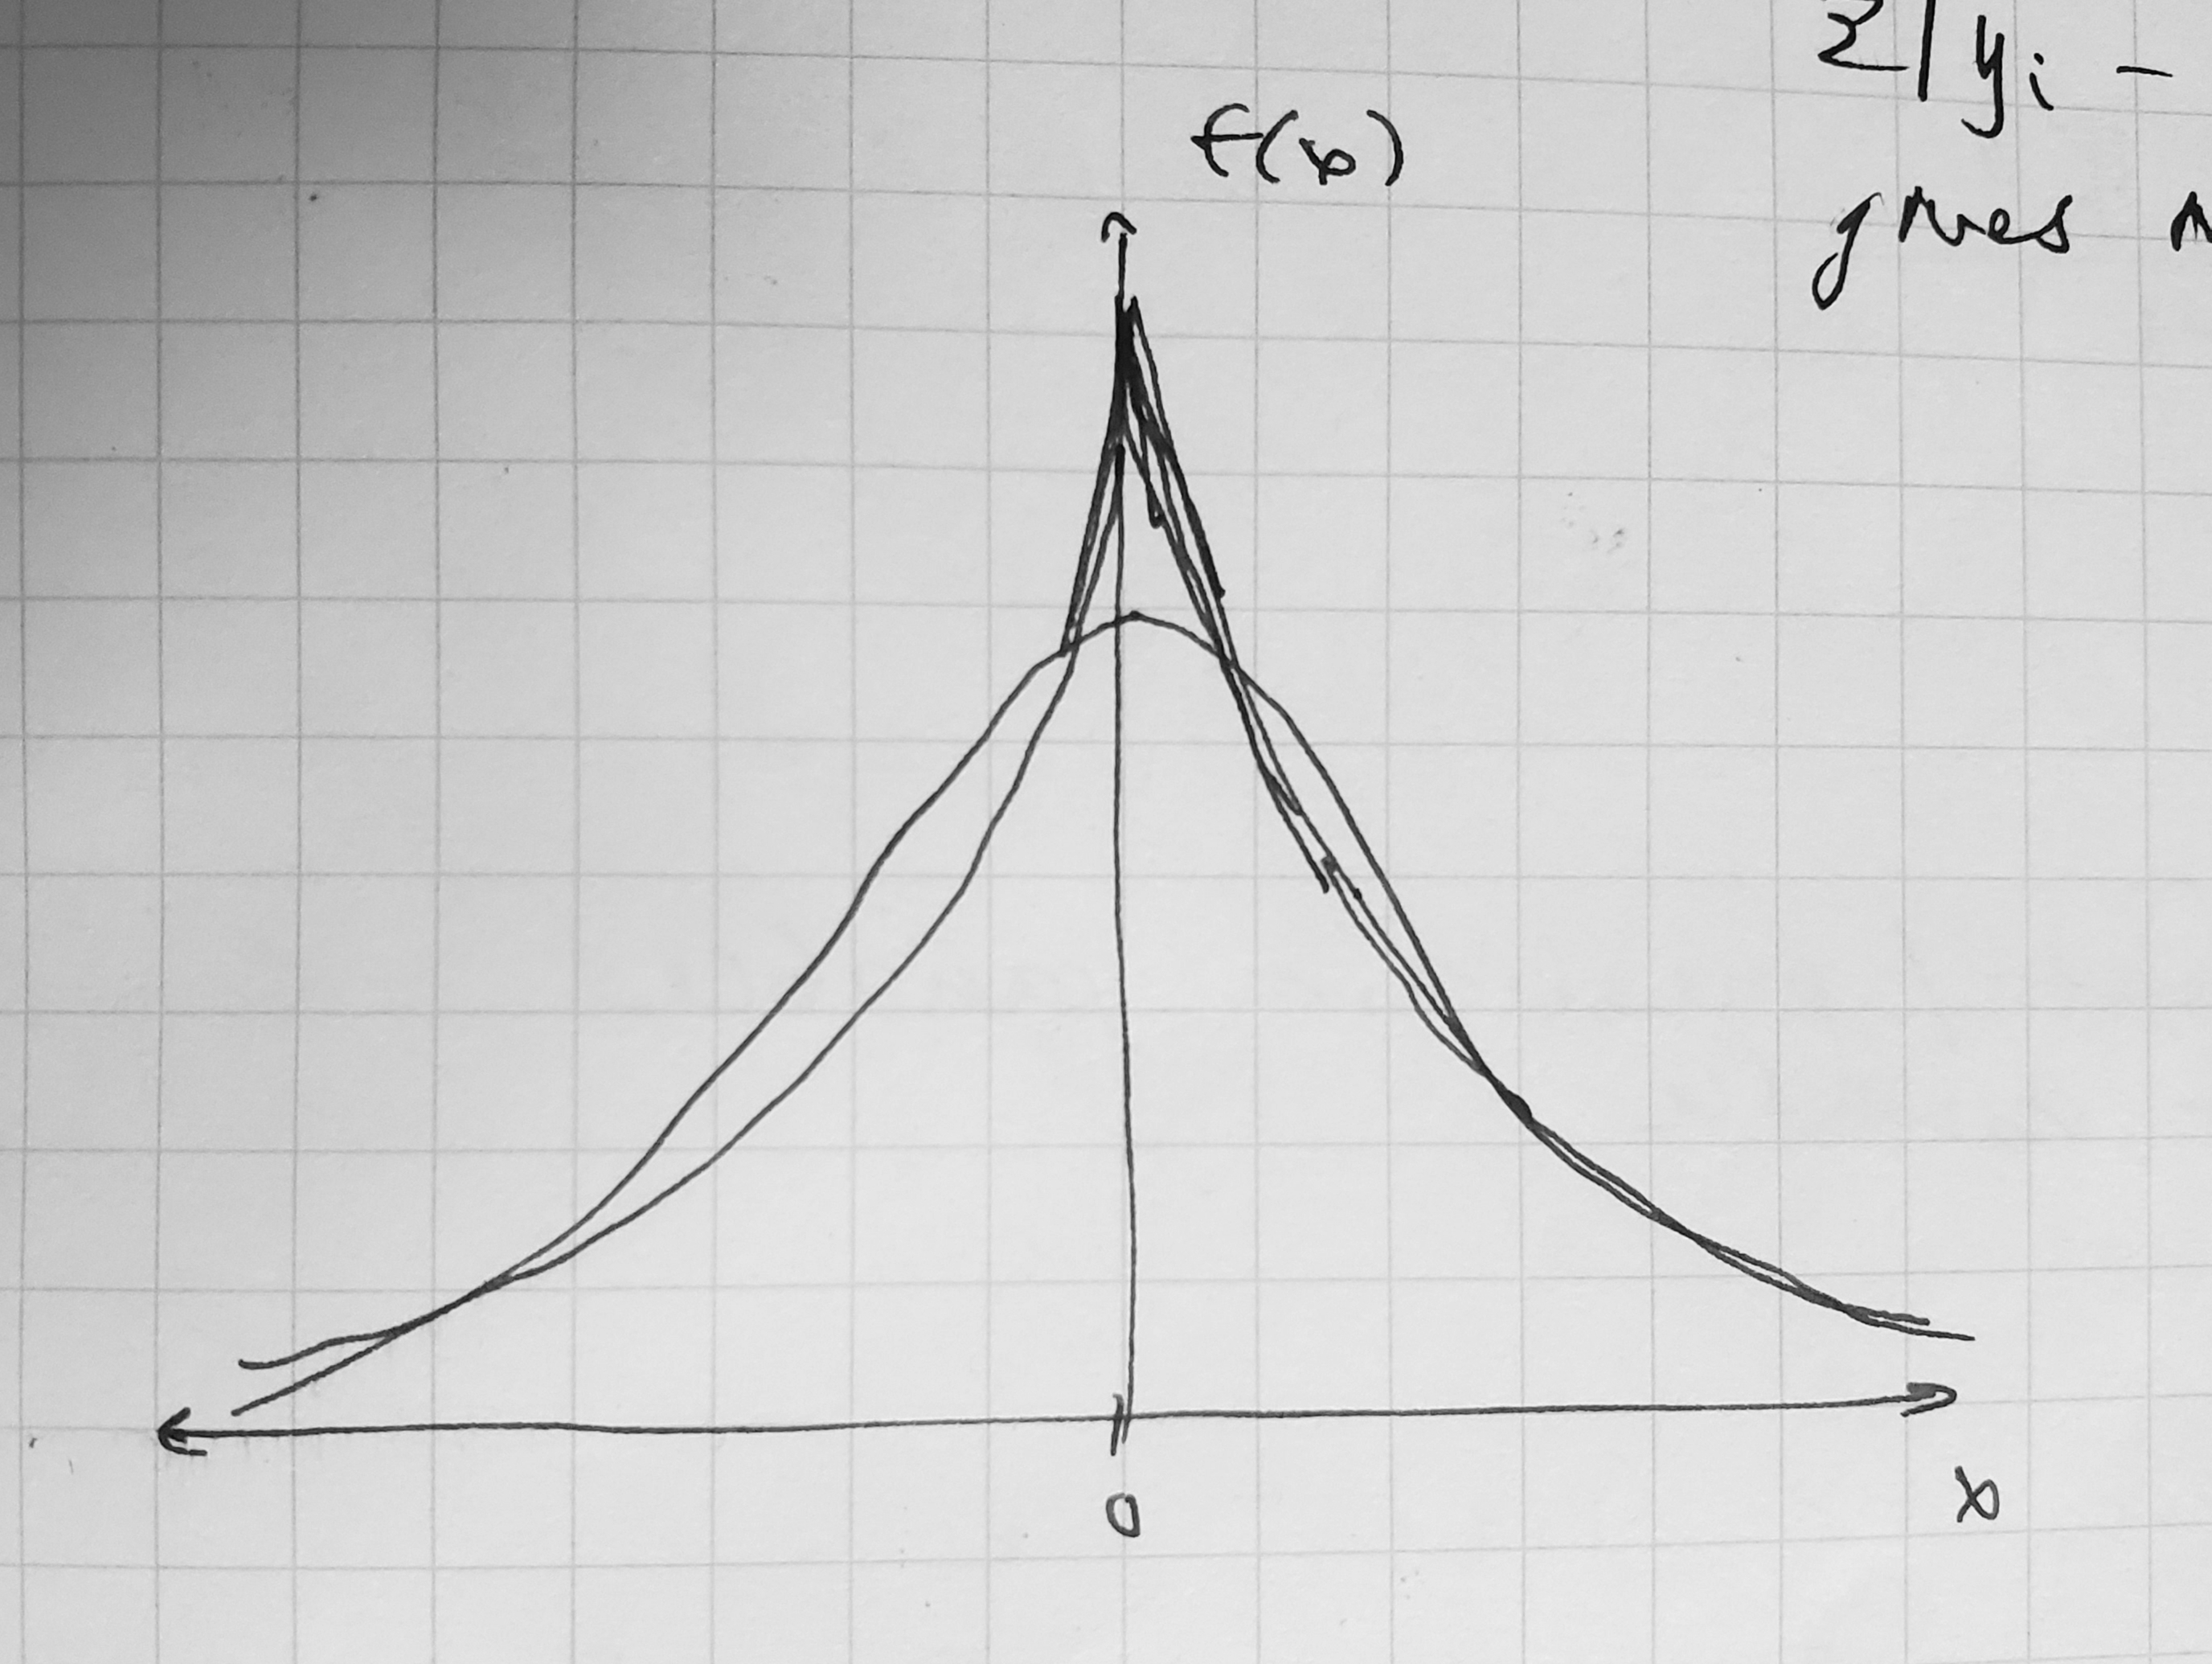
\includegraphics[width=10cm]{q3.jpg}
        \end{figure}

        We see that the Laplace distribution has a sharp peak at $x = 0$ that gives it a higher probability of being exactly 0 than the normal distribution. Hence, the weights are more likely to be exactly 0, and therefore more likely to be sparse.
    \end{solution}

\end{enumerate}

\end{document}